% В этом документе преамбула

%%% Работа с русским языком
\usepackage{cmap}					% поиск в PDF
\usepackage{mathtext} 				% русские буквы в формулах
\usepackage[T2A]{fontenc}			% кодировка
\usepackage[utf8]{inputenc}			% кодировка исходного текста
\usepackage[english,russian]{babel}	% локализация и переносы
\usepackage{indentfirst}			% чтобы первый абзац в разделе отбивался красной строкой
\frenchspacing						% тонкая настройка пробелов

%%% Приведение начертания букв и знаков к русской типографской традиции
\renewcommand{\epsilon}{\ensuremath{\varepsilon}}
\renewcommand{\phi}{\ensuremath{\varphi}}			% буквы "эпсилон"
\renewcommand{\kappa}{\ensuremath{\varkappa}}		% буквы "каппа"
\renewcommand{\le}{\ensuremath{\leqslant}}			% знак меньше или равно
\renewcommand{\leq}{\ensuremath{\leqslant}}			% знак меньше или равно
\renewcommand{\ge}{\ensuremath{\geqslant}}			% знак больше или равно
\renewcommand{\geq}{\ensuremath{\geqslant}}			% знак больше или равно
\renewcommand{\emptyset}{\varnothing}				% знак пустого множества

%%% Дополнительная работа с математикой
\usepackage{amsmath,amsfonts,amssymb,amsthm,mathtools} % AMS
\usepackage{icomma} % "Умная" запятая: $0,2$ --- число, $0, 2$ --- перечисление

%% Номера формул
\mathtoolsset{showonlyrefs=true} % Показывать номера только у тех формул, на которые есть \eqref{} в тексте.

%% Свои команды

% операции, не определённые (или имеющие иные обохначения) в мат. пакетах
\DeclareMathOperator{\sgn}{\mathop{sgn}}				% ф-ия sgn
\renewcommand{\tg}{\mathop{\mathrm{tg}}\nolimits}		% обозначение тангенса

%% Перенос знаков в формулах (по Львовскому)
\newcommand*{\hm}[1]{#1\nobreak\discretionary{}
{\hbox{$\mathsurround=0pt #1$}}{}}

%%% Работа с картинками
\usepackage{graphicx}  % Для вставки рисунков
\graphicspath{{images/}{images2/}}  % папки с картинками
\setlength\fboxsep{3pt} % Отступ рамки \fbox{} от рисунка
\setlength\fboxrule{1pt} % Толщина линий рамки \fbox{}
\usepackage{wrapfig} % Обтекание рисунков текстом

%%% Работа с таблицами
\usepackage{array,tabularx,tabulary,booktabs} % Дополнительная работа с таблицами
\usepackage{longtable}  % Длинные таблицы
\usepackage{multirow} % Слияние строк в таблице

%%% Теоремы
\theoremstyle{plain} % Это стиль по умолчанию, его можно не переопределять.
\newtheorem{theorem}{Теорема}[section]
\newtheorem{lemma}{Лемма}[section]
\newtheorem{definition}[theorem]{Определение}
\newtheorem{property}{Свойство}
 
\theoremstyle{definition} % "Определение"
\newtheorem{corollary}{Следствие}[theorem]
\newtheorem{exmp}{Пример}[section]
 
\theoremstyle{remark} % "Примечание"
\newtheorem*{nonum}{Решение}
\newtheorem*{evidence}{Доказательство}
\newtheorem*{remark}{Примечание}

%%% Программирование
\usepackage{etoolbox} % логические операторы

%%% Страница
\usepackage{extsizes} % Возможность сделать 14-й шрифт
\usepackage{geometry} % Простой способ задавать поля
	\geometry{top=25mm}
	\geometry{bottom=35mm}
	\geometry{left=35mm}
	\geometry{right=20mm}

%\usepackage{fancyhdr} % Колонтитулы
% 	\pagestyle{fancy}
 	%\renewcommand{\headrulewidth}{0pt}  % Толщина линейки, отчеркивающей верхний колонтитул
% 	\lfoot{Нижний левый}
% 	\rfoot{Нижний правый}
% 	\rhead{Верхний правый}
% 	\chead{Верхний в центре}
% 	\lhead{Верхний левый}
%	\cfoot{Нижний в центре} % По умолчанию здесь номер страницы

\usepackage{setspace} % Интерлиньяж (межстрочные интервалы)
%\onehalfspacing % Интерлиньяж 1.5
%\doublespacing % Интерлиньяж 2
%\singlespacing % Интерлиньяж 1

\usepackage{lastpage} % Узнать, сколько всего страниц в документе.

\usepackage{soulutf8} % Модификаторы начертания

\usepackage{hyperref}
\usepackage[usenames,dvipsnames,svgnames,table,rgb]{xcolor}
\hypersetup{				% Гиперссылки
    unicode=true,           % русские буквы в раздела PDF
    pdftitle={Заголовок},   % Заголовок
    pdfauthor={Автор},      % Автор
    pdfsubject={Тема},      % Тема
    pdfcreator={Создатель}, % Создатель
    pdfproducer={Производитель}, % Производитель
    pdfkeywords={keyword1} {key2} {key3}, % Ключевые слова
    colorlinks=true,       	% false: ссылки в рамках; true: цветные ссылки
    linkcolor=MidnightBlue,          % внутренние ссылки
    citecolor=black,        % на библиографию
    filecolor=magenta,      % на файлы
    urlcolor=blue           % на URL
}

\usepackage{csquotes} % Еще инструменты для ссылок

%\usepackage[style=authoryear,maxcitenames=2,backend=biber,sorting=nty]{biblatex}

\usepackage{multicol} % Несколько колонок

%%% Работа с графикой
\usepackage{tikz}
\usetikzlibrary{calc}
\usepackage{tkz-euclide}
\usetikzlibrary{arrows}
\usepackage{pgfplots}
\usepackage{pgfplotstable}

%%% Настройка подписей к плавающим объектам
\usepackage{floatrow}	% размещение
\usepackage{caption}	% начертание
\captionsetup[figure]{labelfont=bf,textfont=it,font=footnotesize}	% нумерация и надпись курсивом
% для подфигур: заголовок подписи полужирный, текст заголовка обычный
% выравнивание является неровным (т.е. выровненным по левому краю)
% singlelinecheck = off означает, что настройка выравнивания используется, даже если заголовок имеет длину только одну строку.
% если singlelinecheck = on, то заголовок всегда центрируется, когда заголовок состоит только из одной строки.
\captionsetup[subfigure]{labelfont=bf,textfont=normalfont,singlelinecheck=off,justification=raggedright}

%%% Stuff для графиков и рисунков



\begin{document}
	
\textit{Почаев Никита Алексеевич, гр. 8381}

\section*{Формула полной вероятности. Формула Байеса. (ДЗ на 29.02.20)}

\subsection*{Задача 1.}

Игровой автомат имеет 3 режима игры:

\begin{table}[h]
	\centering
	\begin{tabular}{|c|c|c|}
		\hline
		Режим                      & \begin{tabular}[c]{@{}c@{}}Вероятность\\ выигрыша\end{tabular} & \begin{tabular}[c]{@{}c@{}}Вероятность\\ выбора режима\end{tabular} \\ \hline
		\RNumb{1} & 0.5                                                            & 0.3                                                                 \\ \hline
		\RNumb{2} & 0.45                                                           & 0.5                                                                 \\ \hline
		\RNumb{3} & 0.4                                                            & 0.2                                                                 \\ \hline
	\end{tabular}
\end{table}

Играем 2 игры. 1-ый вариант - автомат включают заново перед каждой игрой. 2-ой вариант - играем две игры подряд, при этом знает, что режим работы автомата меняется циклически: $1 \to 2 \to 3 \to 1$. Что выгоднее, если цель - два выигрыша?  Старт автомата мы не контролируем.

\textit{Решение:}

\begin{enumerate}
	\item Рассмотрим 1-ый вариант игры. Построим таблицу, где 1-ый шаг - выбор режима, 2-ой - получение / не получение приза.
	\begin{table}[h]
		\centering
		\begin{tabular}{|c|c|c|c|}
			\hline
			$i$                 & \RNumb{1} & \RNumb{2} & \RNumb{3} \\ \hline
			$P(H_i)$            & 0.3                        & 0.5                        & 0.2                        \\ \hline
			$P(A|H_i)=P(B|H_i)$ & 0.5                        & 0.45                       & 0.4                        \\ \hline
		\end{tabular}
	\end{table}
	Перемножаем по колонкам и складываем по столбцам, согласно ФПВ: $P(A) = \sum\limits_{i=1}^{n} P(A|H_i) P(H_i)$.
	\[ P(A) = P(B) = 0.3 \cdot 0.5 + 0.5 \cdot 0.45 + 0.2 \cdot 0.4 = 0.455 \]
	
	Учитывая факт перезапуска автомата для каждой игры, события каждой новой игры можно считать независимыми. Таким образом:
	\[ P(AB) = P(A) \cdot P(B) = 0.207025 \]
	
	\item Рассмотрим 2-ой вариант игры.
	
	Событие $A$ - первая игра была выигрышной. Таблица вероятностей будет аналогична 1-ому пункту: $P(A) = 0.455$. 
	
	Рассмотрим с какой вероятностью выбирается последующий режим игры автомата, если событие $A$ произошло. Вероятности данных событий в сумме дают единицу (4-ого режима или альтернативного выбора $\nexists$), а сами события не пересекаются (не может быть 2 состояния одновременно) $\Rightarrow$ это полная группа событий (ПГС).
	
	\[ P(H_1|A) = \dfrac{P(A|H_1)P(H_1)}{\sum\limits_{i=1}^3 P(A|H_i)P(H_i)} = \dfrac{0.3 \cdot 0.5}{0.3 \cdot 0.5 + 0.5 \cdot 0.45 + 0.2 \cdot 0.4} = 0.3297 \]
	
	Аналогично получаем:
	\[ P(H_2|A) = 0.4945 \]
	\[ P(H_3|A) = 0.1758 \]
	
	Событие $B$ - вторая игра также оказалась выигрышной. Учитывая кольцевую смену режимов аппарата, построим таблицу, по структуре аналогичную предыдущим.
	\begin{table}[h]
		\centering
		\begin{tabular}{|c|c|c|c|}
			\hline
			$i$            & \RNumb{1} & \RNumb{2} & \RNumb{3} \\ \hline
			$P(H_i|A)$       & 0.3297                     & 0.4945                     & 0.1758                     \\ \hline
			$P(B|(H_i|A))$ & 0.45                       & 0.4                        & 0.5                        \\ \hline
		\end{tabular}
	\end{table}

	Выбор следующего режима зависит от предыдущего $\Rightarrow$ все вероятности условные:
	\[ P(B|A) = 0.3297 \cdot 0.45 + 0.4945 \cdot 0.4 + 0.1758 \cdot 0.5 = 0.434 \]
	\[ P(AB) = P(A) \cdot P(B|A) = 0.455 \cdot 0.434 = 0.19747 \]
\end{enumerate}

\textbf{Ответ:} выгоднее каждый раз запускать автомат заново.

\subsection*{Задача 2.}

Белые и чёрные шары распределены по ящикам следующим образом:

\begin{figure}[H]
	\center{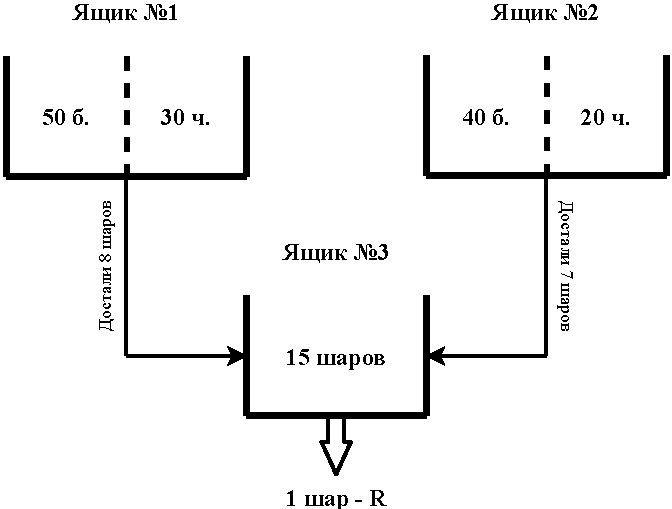
\includegraphics[scale=1]{./media/Homework-29-02-20_1.pdf}}
\end{figure}

\begin{enumerate}
	\item Определить вероятность, что шар $R$ - белый.
	\item Определить вероятность, что в первом ящике осталось 50 белых шаров (т.е. ни одного белого не вытащили), если шар $R$ - белый.
\end{enumerate}

\textit{Решение:}

\begin{enumerate}
	\item Посчитаем вероятности $P(A_i)$ достать $i$ белых шаров из 1-ого ящика. Всего 8 шаров из ящика с 80 шарами можно достать:
	\[ \# \Omega = C_{80}^8 = 28987537150 \]
	способами.
	
	Необходимо рассмотреть все варианты достать шары из ящика. Одним из таких, например, является вариант - 4 белых и 4 чёрных: $\# A_4 = C_{50}^4 \cdot C_{30}^4$.
	
	$A_0 = C_{50}^0 \cdot C_{30}^8 = 1 \cdot 5852925 = 5852925$
	
	$A_1 = C_{50}^1 \cdot C_{30}^7 = 50 \cdot 2035800 = 101790000$
	
	$A_2 = C_{50}^2 \cdot C_{30}^6 = 1225 \cdot 593775 = 727374375$
	
	$A_3 = C_{50}^3 \cdot C_{30}^5 = 19600 \cdot 142506 = 2793117600$
	
	$A_4 = C_{50}^4 \cdot C_{30}^4 = 230300 \cdot 27405 = 6311371500$
	
	$A_5 = C_{50}^5 \cdot C_{30}^3 = 2118760 \cdot 4060 = 8602165600$
	
	$A_6 = C_{50}^6 \cdot C_{30}^2 = 15890700 \cdot 435 = 6912454500$
	
	$A_7 = C_{50}^7 \cdot C_{30}^1 = 99884400 \cdot 30 = 2996532000$
	
	$A_8 = C_{50}^8 \cdot C_{30}^0 = 536878650 \cdot 1 = 536878650$
	
	Соответствующие вероятности событий для 1-ого ящика:
	
	$P(A_0) = \dfrac{A_0}{\# \Omega} = \dfrac{5852925}{28987537150} = 0.000201911772280385$
	
	$P(A_1) = \dfrac{A_1}{\# \Omega} = \dfrac{101790000}{28987537150} = 0.0035115090831371303$
	
	$P(A_2) = \dfrac{A_2}{\# \Omega} = \dfrac{727374375}{28987537150} = 0.025092658656584076$
	
	$P(A_3) = \dfrac{A_3}{\# \Omega} = \dfrac{2793117600}{28987537150} = 0.09635580924128286$
	
	$P(A_4) = \dfrac{A_4}{\# \Omega} = \dfrac{6311371500}{28987537150} = 0.21772706895866797$
	
	$P(A_5) = \dfrac{A_5}{\# \Omega} = \dfrac{8602165600}{28987537150} = 0.29675393102514747$
	
	$P(A_6) = \dfrac{A_6}{\# \Omega} = \dfrac{6912454500}{28987537150} = 0.23846298028806492$
	
	$P(A_7) = \dfrac{A_7}{\# \Omega} = \dfrac{2996532000}{28987537150} = 0.10337311460763406$
	
	$P(A_8) = \dfrac{A_8}{\# \Omega} = \dfrac{536878650}{28987537150} = 0.018521016367201104$
	
	~
	
	Произведём аналогичные расчёты для 2-ого ящика.
	
	Всего 7 шаров из ящика с 60 шарами можно достать: 386206920 способами
	
	Все варианты достать шары из 2-ого ящика:
	
	$B_0 = C_{40}^0 \cdot C_{20}^7 = 1 \cdot 77520 = 77520$
	
	$B_1 = C_{40}^1 \cdot C_{20}^6 = 40 \cdot 38760 = 1550400$
	
	$B_2 = C_{40}^2 \cdot C_{20}^5 = 780 \cdot 15504 = 12093120$
	
	$B_3 = C_{40}^3 \cdot C_{20}^4 = 9880 \cdot 4845 = 47868600$
	
	$B_4 = C_{40}^4 \cdot C_{20}^3 = 91390 \cdot 1140 = 104184600$
	
	$B_5 = C_{40}^5 \cdot C_{20}^2 = 658008 \cdot 190 = 125021520$
	
	$B_6 = C_{40}^6 \cdot C_{20}^1 = 3838380 \cdot 20 = 76767600$
	
	$B_7 = C_{40}^7 \cdot C_{20}^0 = 18643560 \cdot 1 = 18643560$
	
	Соответствующие вероятности событий для 2-ого ящика:
	
	$P(B_0) = \dfrac{B_0}{\# \Omega} = \dfrac{77520}{386206920} = 0.00020072141638477115$
	
	$P(B_1) = \dfrac{B_1}{\# \Omega} = \dfrac{1550400}{386206920} = 0.004014428327695423$
	
	$P(B_2) = \dfrac{B_2}{\# \Omega} = \dfrac{12093120}{386206920} = 0.0313125409560243$
	
	$P(B_3) = \dfrac{B_3}{\# \Omega} = \dfrac{47868600}{386206920} = 0.12394547461759618$
	
	$P(B_4) = \dfrac{B_4}{\# \Omega} = \dfrac{104184600}{386206920} = 0.2697636800500623$
	
	$P(B_5) = \dfrac{B_5}{\# \Omega} = \dfrac{125021520}{386206920} = 0.32371641606007473$
	
	$P(B_6) = \dfrac{B_6}{\# \Omega} = \dfrac{76767600}{386206920} = 0.19877323793162485$
	
	$P(B_7) = \dfrac{B_7}{\# \Omega} = \dfrac{18643560}{386206920} = 0.04827350064053746$
	
	~
	
	В ящике №3 может оказаться от 0 до 15 белых шаров. События вытаскивания из него белого шара $R$ зависит от данного факта. Очевидно, что случае с 0 не рассматривается.
	
	Пусть $\{H_i\}_1^n$ - полная группа события, где $H_i$ - событие, при котором в 3-ем ящике $i$ белых шаров. 
	
	Составим всевозможные комбинации того, как $i$ шаров могут оказаться в 3-ем ящике.
	
	\begin{longtable}[c]{|c|c|c|c|c|c|c|c|c|c|c|}
		\cline{1-2} \cline{4-5} \cline{7-8} \cline{10-11}
		$\mathbf{H_i}$ &
		\textbf{Комбинация событий} &
		&
		$H_4$ &
		\begin{tabular}[c]{@{}c@{}}$(A_0, B_4)$\\ \\ $(A_1, B_3)$\\ \\ $(A_2, B_2)$\\ \\ $(A_3, B_1)$\\ \\ $(A_4, B_0)$\end{tabular} &
		&
		$H_8$ &
		\begin{tabular}[c]{@{}c@{}}$(A_1, B_7)$\\ \\ $(A_2, B_6)$\\ \\ $(A_3, B_5)$\\ \\ $(A_4, B_4)$\\ \\ $(A_5, B_3)$\\ \\ $(A_6, B_2)$\\ \\ $(A_7, B_1)$\\ \\ $(A_8, B_0)$\end{tabular} &
		&
		$H_{12}$ &
		\begin{tabular}[c]{@{}c@{}}$(A_5, B_7)$\\ \\ $(A_6, B_6)$\\ \\ $(A_7, B_5)$\\ \\ $(A_8, B_4)$\end{tabular} \\ \cline{1-2} \cline{4-5} \cline{7-8} \cline{10-11} 
		\endfirsthead
		%
		\endhead
		%
		$H_1$ &
		\begin{tabular}[c]{@{}c@{}}$(A_0, B_1)$\\ \\ $(A_1, B_0)$\end{tabular} &
		&
		$H_5$ &
		\begin{tabular}[c]{@{}c@{}}$(A_0, B_5)$\\ \\ $(A_1, B_4)$\\ \\ $(A_2, B_3)$\\ \\ $(A_3, B_2)$\\ \\ $(A_4, B_1)$\\ \\ $(A_5, B_0)$\end{tabular} &
		&
		$H_9$ &
		\begin{tabular}[c]{@{}c@{}}$(A_2, B_7)$\\ \\ $(A_3, B_6)$\\ \\ $(A_4, B_5)$\\ \\ $(A_5, B_4)$\\ \\ $(A_6, B_3)$\\ \\ $(A_7, B_2)$\\ \\ $(A_8, B_1)$\end{tabular} &
		&
		$H_{13}$ &
		\begin{tabular}[c]{@{}c@{}}$(A_6, B_7)$\\ \\ $(A_7, B_6)$\\ \\ $(A_8, B_5)$\end{tabular} \\ \cline{1-2} \cline{4-5} \cline{7-8} \cline{10-11} 
		$H_2$ &
		\begin{tabular}[c]{@{}c@{}}$(A_0, B_2)$\\ \\ $(A_1, B_1)$\\ \\ $(A_2, B_0)$\end{tabular} &
		&
		$H_6$ &
		\begin{tabular}[c]{@{}c@{}}$(A_0, B_6)$\\ \\ $(A_1, B_5)$\\ \\ $(A_2, B_4)$\\ \\ $(A_3, B_3)$\\ \\ $(A_4, B_2)$\\ \\ $(A_5, B_1)$\\ \\ $(A_6, B_0)$\end{tabular} &
		&
		$H_{10}$ &
		\begin{tabular}[c]{@{}c@{}}$(A_3, B_7)$\\ \\ $(A_4, B_6)$\\ \\ $(A_5, B_5)$\\ \\ $(A_6, B_4)$\\ \\ $(A_7, B_3)$\\ \\ $(A_8, B_2)$\end{tabular} &
		&
		$H_{14}$ &
		\begin{tabular}[c]{@{}c@{}}$(A_7, B_7)$\\ \\ $(A_8, B_6)$\end{tabular} \\ \cline{1-2} \cline{4-5} \cline{7-8} \cline{10-11} 
		$H_3$ &
		\begin{tabular}[c]{@{}c@{}}$(A_0, B_3)$\\ \\ $(A_1, B_2)$\\ \\ $(A_2, B_1)$\\ \\ $(A_3, B_0)$\end{tabular} &
		&
		$H_7$ &
		\begin{tabular}[c]{@{}c@{}}$(A_0, B_7)$\\ \\ $(A_1, B_6)$\\ \\ $(A_2, B_5)$\\ \\ $(A_3, B_4)$\\ \\ $(A_4, B_3)$\\ \\ $(A_5, B_2)$\\ \\ $(A_6, B_1)$\\ \\ $(A_7, B_0)$\end{tabular} &
		&
		$H_{11}$ &
		\begin{tabular}[c]{@{}c@{}}$(A_4, B_7)$\\ \\ $(A_5, B_6)$\\ \\ $(A_6, B_5)$\\ \\ $(A_7, B_4)$\\ \\ $(A_8, B_3)$\end{tabular} &
		&
		$H_{15}$ &
		$(A_8, B_7)$ \\ \cline{1-2} \cline{4-5} \cline{7-8} \cline{10-11} 
	\end{longtable}

	Тогда вероятность каждого события $H_i$ есть сумма вероятностей комбинаций событий, потому что эти комбинации не пересекаются (не могут произойти одновременно):
	
	$P(H_1) = P(A_0) \cdot P(B_1) + P(A_1) \cdot P(B_0) = 8.105603383375651e-07 + 7.04835076815274e-07 = 1.515395415152839e-06$
	
	$P(H_2) = P(A_0) \cdot P(B_2) + P(A_1) \cdot P(B_1) + P(A_2) \cdot P(B_0) = 6.322370639033008e-06 + 1.409670153630548e-05 + 5.0366339864091445e-06 = 2.5455706161747633e-05$
	
	$P(H_3) = 0.00025505367666534906$
	
	$P(H_4) = 0.001705935000371956$
	
	$P(H_5) = 0.008073521060592307$
	
	$P(H_6) = 0.02794557202034627$
	
	$P(H_7) = 0.07208039050283002$
	
	$P(H_8) = 0.1397509646349726$
	
	$P(H_9) = 0.2037671590635703$
	
	$P(H_{10}) = 0.22171508665910591$
	
	$P(H_{11}) = 0.17687347686232707$
	
	$P(H_{12}) = 0.10018528150934262$
	
	$P(H_{13}) = 0.03805480857749707$
	
	$P(H_{14}) = 0.008671664507319158$
	
	$P(H_{15}) = 0.0008940742954654873$
	
	Складывая данные вероятности, получаем $0.999999959471983$, учитывая погрешность округления, данная величина равна единица, что подтверждает верность расчётов и факт того, что данные события являются ПГС.
	
	Событие $P(C)$ - достали белый шар. Составим таблицу с ПГС:
	
	\begin{table}[H]
		\centering
		\resizebox{\textwidth}{!}{%
			\begin{tabular}{|c|c|c|c|c|c|c|c|c|c|c|}
				\cline{1-2} \cline{4-5} \cline{7-8} \cline{10-11}
				$\mathbf{C|H_i}$               & $i$ &  & $\frac{4}{15} =  0.26666666666$ & 4 &  & $\frac{8}{15} =  0.53333333333$  & 8  &  & $\frac{12}{15} =  0.80000000000$ & 12 \\ \cline{1-2} \cline{4-5} \cline{7-8} \cline{10-11} 
				$\frac{1}{15} = 0.06666666666$ & 1   &  & $\frac{5}{15} =  0.33333333333$ & 5 &  & $\frac{9}{15} =  0.60000000000$  & 8  &  & $\frac{13}{15} =  0.86666666666$ & 13 \\ \cline{1-2} \cline{4-5} \cline{7-8} \cline{10-11} 
				$\frac{2}{15} = 0.13333333333$ & 2   &  & $\frac{6}{15} =  0.40000000000$ & 6 &  & $\frac{10}{15} =  0.66666666666$ & 10 &  & $\frac{14}{15} =  0.93333333333$ & 14 \\ \cline{1-2} \cline{4-5} \cline{7-8} \cline{10-11} 
				$\frac{3}{15} = 0.20000000000$ & 3   &  & $\frac{7}{15} =  0.46666666666$ & 7 &  & $\frac{11}{15} =  0.73333333333$ & 11 &  & $\frac{15}{15} =  1.00000000000$ & 15 \\ \cline{1-2} \cline{4-5} \cline{7-8} \cline{10-11} 
			\end{tabular}%
		}
	\end{table}

	\[ P(C) = \sum_{i=1}^{15} P(H_i)P(C|H_i) = 0.6444444444444444 \]
	
	\textbf{2-ой вариант решения (КРАТКИЙ)}
	
	Пусть событие $A$ - в итоге вытащен белый шар.
	
	Пусть события $H_i$ - вытащенный шар был в $i$-ом ящике. Тогда они образуют ПГС.
	
	\begin{table}[h]
		\centering
		\begin{tabular}{|c|c|c|}
			\hline
			$i$        & 1               & 2               \\ \hline
			$P(H_i)$   & $\frac{8}{15}$  & $\frac{7}{15}$  \\ \hline
			$P(A|H_i)$ & $\frac{50}{80}$ & $\frac{40}{60}$ \\ \hline
		\end{tabular}
	\end{table}

	\[ P(A) = \dfrac{8}{15} \cdot \dfrac{50}{80} + \dfrac{7}{15} \cdot \dfrac{40}{60} = 0.6444444 \]
	
	\item Если в 1-м ящике осталось 50 белых шаров, то из него \underline{не взяли ни одного белого}. Тогда белых в третьем ящике может быть от от 1 до 7 (не 0, потому что из него достали белый шар), так как они все из второго ящика.
	
	Таким образом, надо посчитать:
	
	\[ P(H_1|C) = \dfrac{P(H_1) \cdot P(C|H_1)}{P(C)} = \dfrac{1.515395415152839e-06 \cdot 0.06666666666}{0.6444444} = 2.633348913284238e-06 \]
	\[ P(H_2|C) = 5.276972620662395e-05 \]
	\[ P(H_3|C) = 0.0005294281035637105 \]
	\[ P(H_4|C) = 0.0033407673354175073 \]
	\[ P(H_5|C) = 0.014454606217420484 \]
	\[ P(H_6|C) = 0.044739552725894506 \]
	\[ P(H_7|C) = 0.10119897439084223 \]
	
	В таблице комбинаций, составленной в предыдущем пункте теперь нас интересуют лишь пункты $H_1 - H_7$ (в них содержится $A_0$ - благоприятное для нас событие).
	
	Учитывая способ вычисления при помощи таблицы для ПГС, получаем вывод, что $A_0 - A_7$ образуют ПГС: чтобы выполнилось $H_1$ при $A_0$ нужен $B_1$, а при $A_1$ нужен $B_0$. Если пары нет, то вероятность $P(H_1|A_i) = 0$. На основе этого получаем таблицу:
	
	\begin{table}[H]
		\centering
		\begin{tabular}{|c|c|c|c|c|c|c|c|c|}
			\hline
			$i$          & 0                            & 1                             & 2   & 3   & 4   & 5   & 6   & 7   \\ \hline
			$P(A_i)$     & 0.000201911772280385         & 0.0035115090831371303         & ... & ... & ... & ... & ... & ... \\ \hline
			$P(H_1|A_i)$ & $= P(B_1) = $ 0.004014428... & $= P(B_0) = $0.00020072141... & 0   & 0   & 0   & 0   & 0   & 0   \\ \hline
		\end{tabular}
	\end{table}

	Выражаем:
	\[ P(A_0|H_1) = \dfrac{P(H_1|A_0) \cdot P(A_0)}{\sum\limits_{i=0}^{7} P(H_1|A_i) P(A_i)} = \dfrac{P(H_1|A_0) \cdot P(A_0)}{P(H_1)} = 0.5348837209302326 \]
	
	Таким образом, получаем:
	\[ P(A_0|(H_1|C)) = P(A_0|H_1) \cdot P(H_1|C) = 0.5348837209302326 \cdot 2.633348913284238e-06 = \]
	\[ = 1.4085354652450578e-06 \]
	
	Пользуясь аналогичными рассуждениям для $H_2 - H_7$ получаем:
	
	\[ P(A_0|H_2) = \dfrac{P(H_1|A_0) \cdot P(A_0)}{P(H_2)} = \dfrac{P(B_2) \cdot P(A_0)}{P(H_2)} = 0.2483675211703085 \]
	\[ P(A_0|(H_2|C)) = P(A_0|H_2) \cdot P(H_2|C) = 1.3106286090775058e-05 \]
	
	\[ P(A_0|H_3) = 0.09812072020827407 \]
	\[ P(A_0|(H_3|C)) = 5.194786682017199e-05 \]
	
	\[ P(A_0|H_4) = 0.031928803104403575 \]
	\[ P(A_0|(H_4|C)) = 0.00010666670247016857 \]
	
	\[ P(A_0|H_5) = 0.008095867316428222 \]
	\[ P(A_0|(H_5|C)) = 0.00011702257404745466 \]
	
	\[ P(A_0|H_6) = 0.0014361723110718318 \]
	\[ P(A_0|(H_6|C)) = 6.425370683466798e-05 \]
	
	\[ P(A_0|H_7) = 0.00013522385215333335 \]
	\[ P(A_0|(H_7|C)) = 1.3684515151096217e-05 \]
	
	\[ P(A_0|C) = P(A_0|(H_1|C)) + \dots + P(A_0|(H_7|C)) = 0.00036809018687957953 (\textbf{???}) \]
	
	\textbf{2-ой вариант решения (КРАТКИЙ)}

	Обратимся к таблице из 1-ого пункт: $H_2$ - событие, при котором белый шар, вытащенный из 3-его ящика изначально находился во 2-ом. Тогда:
	\[ P(H_2|A) = \dfrac{P(A|H_2)P(H_2)}{P(A)} = \dfrac{\frac{40}{60} \cdot \frac{7}{15}}{\frac{29}{45}} = \dfrac{14}{29} \approx 0.482759 \]
	
	Событие $B$ - из 1-ого ящика вынули 8 чёрных шаров (т.е. ни одного белого).
	
	\[ P(B) = \dfrac{C_{30}^8}{C_{80}^8} = \dfrac{5852925}{28987537150} \approx 0.000202 \]
	
	Тогда вероятность, что в 1-м ящике осталось 50 белых, при условии, что из 3-го ящика вытащили белый шар, который изначально был во 2-ом:
	\[ P(B|(H_2|A)) = 0.000202 \cdot 0.482759 \approx 0.000098 \]
\end{enumerate}

\subsection*{Задача 3.}

Белые и чёрные шары распределены по ящикам следующим образом:

\begin{figure}[H]
	\center{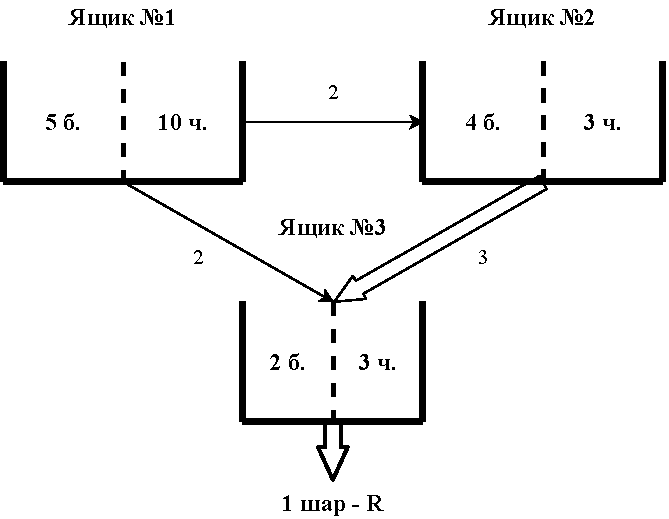
\includegraphics[scale=1]{./media/Homework-29-02-20_2.pdf}}
\end{figure}

\begin{enumerate}
	\item Определить вероятность, что вытащенный шар $R$ белый
	\item Если вытащенный шар белый, определить вероятность, что в 3-м ящике осталось 2 белых
	\item Если вытащенный шар белый, определить вероятность, что из 2-го ящика в 3-й переложены все белые
\end{enumerate}

\textit{Решение:}

\begin{enumerate}
\item События $A_i, 0 \le i \le 2$ - из 1-ого ящика в 3-ий переложили $i$ белых шаров образуют ПГС. Всего возможных вариантов данного действия: $C_{15}^2 = 105$.

	События $B_j, 0 \le j \le 2$ - из 1-го ящика во 2-й переложили $j$ белых шаров.
	
	Построим таблицу условных вероятностей для каждого $B_j$-ого. Всего вариантов данного события (учитывая, что два уже вытащены из 1-го ящика): $C_{13}^2 = 78$. Если, например, из 1-го ящика в 3-й переложили 1 белый, то в 1-м ящике осталось 4 белых и 9 черных.
	
	\begin{table}[h]
		\centering
		\begin{tabular}{|c|c|c|c|}
			\hline
			$i$          & 0                                                      & 1                                                       & 2                                                       \\ \hline
			$P(A_i)$     & $\frac{C_5^0 \cdot C_{10}^2}{C_{15}^2} = \frac{3}{7}$  & $\frac{C_5^1 \cdot C_{10}^1}{C_{15}^2} = \frac{10}{21}$ & $\frac{C_5^2 \cdot C_{10}^0}{C_{15}^2} = \frac{2}{21}$  \\ \hline
			$P(B_0|A_i)$ & $\frac{C_5^0 \cdot C_{8}^2}{C_{13}^2} = \frac{14}{39}$ & $\frac{C_4^0 \cdot C_{9}^2}{C_{13}^2} = \frac{6}{13}$   & $\frac{C_3^0 \cdot C_{10}^2}{C_{13}^2} = \frac{15}{26}$ \\ \hline
			$P(B_1|A_i)$ & $\frac{C_5^1 \cdot C_{8}^1}{C_{13}^2} = \frac{20}{39}$ & $\frac{C_4^1 \cdot C_{9}^1}{C_{13}^2} = \frac{6}{13}$   & $\frac{C_3^1 \cdot C_{10}^1}{C_{13}^2} = \frac{5}{13}$  \\ \hline
			$P(B_2|A_i)$ & $\frac{C_5^2 \cdot C_{8}^0}{C_{13}^2} = \frac{5}{39}$  & $\frac{C_4^2 \cdot C_{9}^0}{C_{13}^2} = \frac{1}{13}$   & $\frac{C_3^2 \cdot C_{10}^0}{C_{13}^2} = \frac{1}{26}$  \\ \hline
		\end{tabular}
	\end{table}
	
	По формуле ПГС найдём вероятности $P(B_0), P(B_1), P(B_2)$:
	
	\[ P(B_0) = \sum_{i=0}^{2} P(B_0|A_i) \cdot P(A_i) = \dfrac{3}{7} \]
	\[ P(B_1) = \sum_{i=0}^{2} P(B_1|A_i) \cdot P(A_i) = \dfrac{10}{21} \]
	\[ P(B_2) = \sum_{i=0}^{2} P(B_2|A_i) \cdot P(A_i) = \dfrac{2}{21} \]
	
	Видно, что вероятности $B_0, B_1, B_2$ также образуют ПГС.
	
	События $C_k$ - из 2-го ящика в 3-й переложили k белых шаров.
	
	\begin{table}[h]
		\centering
		\begin{tabular}{|c|c|c|c|}
			\hline
			$B_i$        & $B_0$                                             & $B_1$                                             & $B_2$                                             \\ \hline
			$P(B_i)$     & $\frac{3}{7}$                                     & $\frac{10}{21}$                                   & $\frac{2}{21}$                                    \\ \hline
			$P(C_0|B_i)$ & $\frac{C_4^0 \cdot C_5^3}{C_9^3} = \frac{5}{42}$  & $\frac{C_5^0 \cdot C_4^3}{C_9^3} = \frac{1}{21}$  & $\frac{C_6^0 \cdot C_3^3}{C_9^3} = \frac{1}{84}$  \\ \hline
			$P(C_1|B_i)$ & $\frac{C_4^1 \cdot C_5^2}{C_9^3} = \frac{10}{21}$ & $\frac{C_5^1 \cdot C_4^2}{C_9^3} = \frac{5}{14}$  & $\frac{C_6^1 \cdot C_3^2}{C_9^3} = \frac{3}{14}$  \\ \hline
			$P(C_2|B_i)$ & $\frac{C_4^2 \cdot C_5^1}{C_9^3} = \frac{5}{14}$  & $\frac{C_5^2 \cdot C_4^1}{C_9^3} = \frac{10}{21}$ & $\frac{C_6^2 \cdot C_3^1}{C_9^3} = \frac{15}{28}$ \\ \hline
			$P(C_3|B_i)$ & $\frac{C_4^3 \cdot C_5^0}{C_9^3} = \frac{1}{21}$  & $\frac{C_5^3 \cdot C_4^0}{C_9^3} = \frac{5}{42}$  & $\frac{C_6^3 \cdot C_3^0}{C_9^3} = \frac{5}{21}$  \\ \hline
		\end{tabular}
	\end{table}
	
	По формуле ПГС найдём вероятности $P(C_0), P(C_1), P(C_2), P(C_3)$:
	
	\[ P(C_0) = \sum_{i=0}^{2} P(C_0|B_i) \cdot P(B_i) = \dfrac{11}{147} \]
	\[ P(C_1) = \sum_{i=0}^{2} P(C_1|B_i) \cdot P(B_i) = \dfrac{58}{147} \]
	\[ P(C_2) = \sum_{i=0}^{2} P(C_2|B_i) \cdot P(B_i) = \dfrac{190}{441} \]
	\[ P(C_3) = \sum_{i=0}^{2} P(C_3|B_i) \cdot P(B_i) = \dfrac{44}{441} \]
	
	\[ \sum_{i=0}^{3} P(C_i) = 1 \Rightarrow \text{ события образуют ПГС} \]
	
	Событие $D_l$ – в 3-й ящик попало $l$ белых (из 1-го и 2-го ящика).
	
	\begin{table}[h]
		\centering
		\begin{tabular}{|c|c|c|c|c|c|c|}
			\hline
			$l$                & 0            & 1                                                                      & 2                                                                                        & 3                                                                                        & 4                                                                      & 5            \\ \hline
			Комбинация событий & $(C_0, A_0)$ & \begin{tabular}[c]{@{}c@{}}$(C_1, A_0)$\\ \\ $(C_0, A_1)$\end{tabular} & \begin{tabular}[c]{@{}c@{}}$(C_2, A_0)$\\ \\ $(C_1, A_1)$\\ \\ $(C_0, A_2)$\end{tabular} & \begin{tabular}[c]{@{}c@{}}$(C_3, A_0)$\\ \\ $(C_2, A_1)$\\ \\ $(C_1, A_2)$\end{tabular} & \begin{tabular}[c]{@{}c@{}}$(C_3, A_1)$\\ \\ $(C_2, A_2)$\end{tabular} & $(C_3, A_2)$ \\ \hline
		\end{tabular}
	\end{table}
	
	\[ P(D_0) = P(C_0) \cdot P(A_0) = 0.032 \]
	\[ P(D_1) = P(C_1) \cdot P(A_0) + P(C_0) \cdot P(A_1) = 0.204 \]
	\[ P(D_2) = P(C_2) \cdot P(A_0) + P(C_1) \cdot P(A_1) + P(C_0) \cdot P(A_2) = 0.379 \]
	\[ P(D_3) = P(C_3) \cdot P(A_0) + P(C_2) \cdot P(A_1) + P(C_1) \cdot P(A_2) = 0.2855 \]
	\[ P(D_4) = P(C_3) \cdot P(A_1) + P(C_2) \cdot P(A_2) = 0.0885 \]
	\[ P(D_5) = P(C_3) \cdot P(A_2) = 0.0095 \]
	
	\[ \sum_{i=0}^{5} P(D_i) \approx 1 \Rightarrow \text{ события образуют ПГС} \]
	
	В результате в 3-ем ящике 10 шаров.
	
	Событие $E$ - из 3-го ящика достали белый шар.
	
	\begin{table}[h]
		\centering
		\begin{tabular}{|c|c|c|c|c|c|c|}
			\hline
			$i$        & 0              & 1              & 2              & 3              & 4              & 5              \\ \hline
			$P(D_i)$   & 0.032          & 0.204          & 0.379          & 0.2855         & 0.0885         & 0.0095         \\ \hline
			$P(E|D_i)$ & $\frac{2}{10}$ & $\frac{3}{10}$ & $\frac{4}{10}$ & $\frac{5}{10}$ & $\frac{6}{10}$ & $\frac{7}{10}$ \\ \hline
		\end{tabular}
	\end{table}
	
	\[ P(E) = \sum_{i=0}^{5} P(D_i)P(E|D_i) = 0.4217 \]
	
	\item Если в 3-м ящике 2 белых, то в него не добавилось ни одного белого, что соответствует событию $D_0$:
	
	\[ P(D_0|E) = \dfrac{P(E|D_0) \cdot P(D_0)}{P(E)} = 0.01517 \]
	
	\item То, что в 3-й ящик из 2-го переложены все белые, соответствует событию $C_3$. Это может возникнуть при $D_3, D_4, D_5$.
	
	\[ P(D_3|E) = \dfrac{P(E|D_3) \cdot P(D_3)}{P(E)} = 0.3385 \]
	\[ P(D_4|E) = \dfrac{P(E|D_4) \cdot P(D_4)}{P(E)} = 0.1259 \]
	\[ P(D_5|E) = \dfrac{P(E|D_5) \cdot P(D_5)}{P(E)} = 0.01577 \]
	
	Запишем таблицу комбинаций, аналогичную таблице из 2-ого пункта 2-ой задачи ($D_i$ в ПГС $C_i$).
	
	\begin{table}[h]
		\centering
		\begin{tabular}{|c|c|c|c|c|}
			\hline
			$i$          & 0                & 1                & 2                 & 3                \\ \hline
			$P(C_i)$     & $\frac{11}{147}$ & $\frac{58}{147}$ & $\frac{190}{441}$ & $\frac{44}{441}$ \\ \hline
			$P(D_3|C_i)$ & 0                & $P(A_2)$         & $P(A_1)$          & $P(A_0)$         \\ \hline
			$P(D_4|C_i)$ & 0                & 0                & $P(A_2)$          & $P(A_1)$         \\ \hline
			$P(D_5|C_i)$ & 0                & 0                & 0                 & $P(A_2)$         \\ \hline
		\end{tabular}
	\end{table}

	\[ P(C_3|D_3) = \dfrac{P(C_3) \cdot P(D_3|C_3)}{P(D_3)} = \dfrac{P(C_3) \cdot P(A_0)}{P(D_3)} = 0.14977 \]
	\[ P(C_3|D_4) = \dfrac{P(C_3) \cdot P(A_1)}{P(D_4)} = 0.5368 \]
	\[ P(C_3|D_5) = 1 \]
	
	\[ P(C_3|E) = P(C_3|D_3) \cdot P(D_3|E) + P(C_3|D_4) \cdot P(D_4|E) + P(C_3|D_5) \cdot P(D_5|E) = \]
	\[ = 0.14977 \cdot 0.3385 + 0.5368 \cdot 0.1259 + 1 \cdot 0.01577 = 0.134 \]
\end{enumerate}

\subsection*{Задача 3. (Решение от Малова)}

Белые и чёрные шары распределены по ящикам следующим образом:

\begin{figure}[H]
	\center{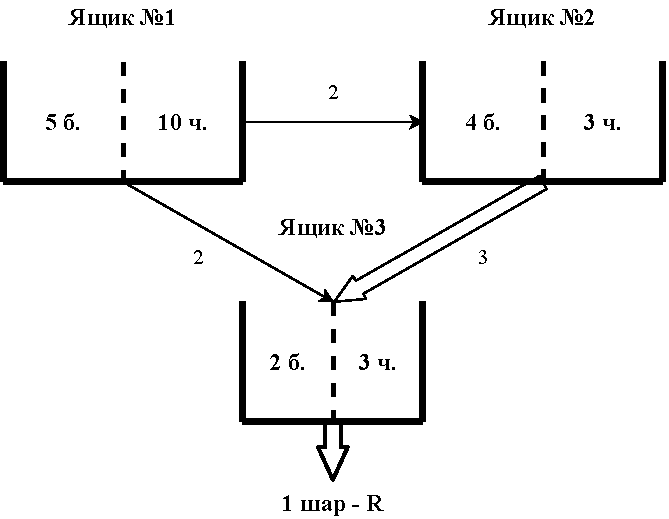
\includegraphics[scale=1]{./media/Homework-29-02-20_2.pdf}}
\end{figure}

\begin{enumerate}
	\item Определить вероятность, что вытащенный шар $R$ белый
	\item Если вытащенный шар белый, определить вероятность, что в 3-м ящике осталось 2 белых
	\item Если вытащенный шар белый, определить вероятность, что из 2-го ящика в 3-й переложены все белые
\end{enumerate}

\textit{Решение:}

Отслеживаем, как белые шары двигались по ящикам.

\begin{itemize}
	\item Событие $A$ - вытащен белый шар. 
	\item Событие $H_i$ - вытащенный шар изначально был в $i$-ом ящике, $i=1,2,3$.
	\item $B_j$ - вытащенный шар пришёл в 3-ий из $j$-ого, $j=1,2,3$.
\end{itemize}

\begin{table}[h]
	\centering
	\begin{tabular}{|c|c|c|}
		2 шара из 1-ого ящ. & 3 шара из 2-ого ящ. & 5 шаров было в 3-ем \\ \hline
	\end{tabular}
\end{table}

Считаем вероятности $B_j$: 

\begin{table}[h]
	\centering
	\begin{tabular}{cccc}
		\hline
		\multicolumn{1}{|c|}{$i$}        & \multicolumn{1}{c|}{1}              	   & \multicolumn{1}{c|}{2}                  & \multicolumn{1}{c|}{3}              \\ \hline
		\multicolumn{1}{|c|}{$P(B_j)$}   & \multicolumn{1}{c|}{$\nicefrac{2}{10}$} & \multicolumn{1}{c|}{$\nicefrac{3}{10}$} & \multicolumn{1}{c|}{$\nicefrac{5}{10}$} \\ \hline
		\multicolumn{1}{|c|}{$P(A|B_j)$} & \multicolumn{1}{c|}{$?$}                & \multicolumn{1}{c|}{$?$}                & \multicolumn{1}{c|}{$\nicefrac{2}{5}$}  \\ \hline
		& $\nicefrac{1}{3}$              &  $\nicefrac{4}{7}$                      &                                    
	\end{tabular}
\end{table}

Если белый шар пришёл из 1-ого ящика, то он однозначно изначально был в нём. Значит, из $B_1 \Rightarrow H_1$.

\begin{figure}[H]
	\center{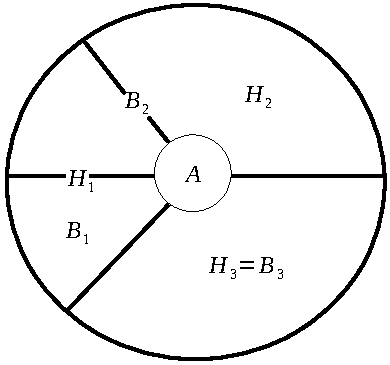
\includegraphics[scale=1]{./media/Homework-29-02-20_3.pdf}}
\end{figure}

Дозаполняем таблицу:

\begin{enumerate}
	\item Необходимо вычислить вероятность $P(A|B_j) = \dfrac{P(AB_j)}{P(B_j)}$
	
	\[ P(AB_1) = P(AB_1H_1) = \underset{=\frac{5}{15}=\frac{1}{3}}{P(A|B_1H_1)} \cdot \underset{=1}{P(H_1|B_1)} \cdot P(B_1) \]
	
	$P(A|B_1H_1) = \frac{5}{15}$, т.к. по сути это события, что вытащен один из 2-х шаров, что мы перекладывали из 1-ого ящика во 2-ой.
	
	\item $P(AB_2) = \dots$
\end{enumerate}

Построим иную таблицу с более удобным (хронологически) порядком:

\begin{table}[H]
	\centering
	\begin{tabular}{|c|c|c|c|}
		\hline
		$i$        & 1             & 2             & 3              \\ \hline
		$P(H_i)$   & $?$           & $?$           & $\frac{5}{10}$ \\ \hline
		$P(A|H_i)$ & $\frac{1}{3}$ & $\frac{4}{7}$ & $\frac{2}{5}$  \\ \hline
	\end{tabular}
\end{table}

\[ P(H_1) = P(BH_1) + P(B_2H_1) = \underset{=1}{P(H_1|B_1)} \underset{=0.2}{P(B_1)} + \underset{=\frac{2}{9}}{P(H_1|B_2)} \underset{=\frac{3}{10}}{P(B_2)} \]

\[ P(H_2) = P(H_2|B_2) P(B_2) = \frac{7}{9} \cdot \frac{3}{10} = \frac{7}{30} \]

\[ P(H_1) = \frac{2}{10} + \frac{2}{3} \cdot \frac{3}{10} = \frac{8}{30} \]

В результате для первой строки нашей последней таблицы получаем:

\[ \frac{8}{30} + \frac{7}{30} + \underset{=\frac{15}{30}}{\frac{15}{30}} = 1 \]
Т.е. всё верно и вычисления 3-ей величины мы производили для проверки. 

\end{document} 